\documentclass{standalone}

\usepackage{tikz}
\usetikzlibrary{matrix,positioning,shapes.arrows,fit}

\begin{document}
	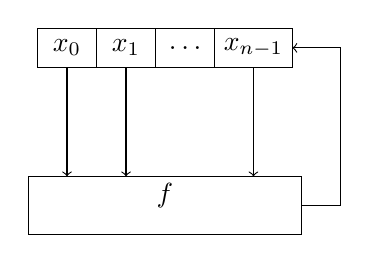
\begin{tikzpicture}[
		every node/.style = {
			draw, rectangle, 
			minimum width=0.75cm,
			minimum height=0.5cm,
			outer sep=0cm, 
			%inner sep=0cm,
			node distance=0cm
			}
		]
		\node (x0) {$x_0$};
		\node [right=of x0.east] (x1) {$x_1$};
		\node [right=of x1.east] (tmp) {$\ldots$};
		\node [right=of tmp.east] (xn1) {$x_{n-1}$};
		
		\node [below=2cm of tmp, fit=(x0)(xn1)] (f) {$f$};
		
		\draw[->] (x0.south) -- (x0.south |- f.north);
		\draw[->] (x1.south) -- (x1.south |- f.north);
		\draw[->] (xn1.south) -- (xn1.south |- f.north);
		
		\draw[->] (f.east) -| ++(0.5,0) |- (xn1.east);
		
	\end{tikzpicture}
\end{document}